\section{Dynamic Programming III}

We'll look at more examples today of DP.

\subsection{Knapsack (without repetition)}
\begin{itemize}
	\item Start with a recap with knapsack: had a weight capacity $W$, and a set of items with individual 
		weights $(w_i, v_i)$, and we wanted to look at the most valuable combination of items.
	\item Now, we're going to look at this problem with the with the constraint that \textit{we cannot 
		choose with repetition}
	\item To solve, look at how we solved the problem with repetition: introduced $K(c)$ which gets us 
		the best achieveable value for a capacity $c \le W$. The issue with trying the same thing 
		is that our subproblems don't track which items have already been used. Why not keep track of both? 
\end{itemize}

\subsubsection{Subproblems}
\begin{itemize}
	\item Introduce a 2D array: essentially solve the problem for smaller knapsacks and also smaller 
		capacities. Then expand in two directions: in terms of the number of items and also the 
		capacity.
	\item So keep track of all weights $c \le W$ and all items $j \le n$. Define $K(j, c)$ to be the 
		optimal solution to the knapsack for capacity $c$ and items $\{1, 2, \dots, j\} $. (It doesn't 
		need to use all the items from 1 to $j$.
	\item For each $K(j, c)$, we recurse smaller subproblems:

		\textit{Case 1:} The optimal solution on items 1 through $j$ doesn't use item $j$. 
					Here, $K(j, c) = K(j-1, c)$.

			\comment{Note that this is not equivalent to $K(j-1, c - w_j)$, since the $w_j$ could be 
			distributed among other items.}

		\textit{Case 2:} the optimal solution on items 1 through $j$ uses item $j$.
		Here, $K(j, c) = K(j-1, c - w_j) + v_j$. We add $v_j$ to $K$ since we're now using item $j$.   

		The intuition here is that we use the optimal solution without item $j$, then add in item $j$ 
		at the end. 
\end{itemize}
\subsubsection{Implementation}
\begin{itemize}
	\item So let's formalize this:
		\[
			K(j, c) = \max\{ K(j-1, c), v_j + K(j-1, c - w_j)\}
		.\]
		with base cases $K(0, c) = 0$ and $K(j, 0) = 0$. The base cases make sense since with no items our 
		optimal value is 0, and with no allowed weights then the optimal value is also 0. 

	\item Looking at $K(j, c)$ it only relies on the subproblmes $K(j-1, c)$, or $K(j-1, c - w_j)$, so we're 
		only looking at row $j-1$, and different elements in that row. This tells us about the order in which 
		we should be solving the subproblems: we could either do this row by row or column by column. 
	\item For runtime, ther eare $O(nW)$ subproblems, and in each subproblem we're doing constant 
		work (memory access), so therefore the total runtime is $O(nW)$, just like knapsack with repetition. 
	\item For space complexity, notice that each $K$ only depends on the previous row, so once we've 
		moved onto the 3rd row, we no longer need the first. We can delete this from memory, so the optimized 
		space complexity is $O(W)$. 
\end{itemize}
\subsection{Traveling Salesperson Problem}
\begin{itemize}
	\item A notoriously difficult problem, and DP helps us get a \textit{slightly} better runtime. 
	\item Input: Cities $1, \dots, n$ and pairwise distances $d_{ij}$ between cities $i$ and $j$. We want to 
		find a ``tour'' of minimum total distance (so we need to visit every city exactly once and 
		return to the city we started at).
	\item The naive brute-force algorithm basically is the one where we have to go through all possible 
		tours: there are \( n! \in O(n^n) \) possible tours, which makes this computation very expensive. 
	\item Dynamic programming gives us $O(n^2 2^n)$. (this is nearly optimal, beating $O(n 2^n)$ is theorized
		to be impossible)
		\begin{itemize}
			\item To give an illustration of the difference DP makes, if $n = 25$, then $O(n!) \approx 10^{25}$, 
				whereas $O(n^2 2^n) \approx 10^{10}$, so we're already better by 15 orders of magnitude. 
		\end{itemize}
\end{itemize}
\subsubsection{Subproblems}
\begin{itemize}
	\item One challenge of TSP is that subproblems aren't exactly solving the problem. If we just look at 
		TSP for a subset of our graph, that doesn't necessarily give us a solution to the larger problem, since 
		we're looking for cycles. Instead, we think of ``partial solutions'' to our graph. 
	\item We think of the subproblmes as starting from city 1, ends in city $j$, and passes thorugh all cities
		in a set $S$ (which includes city 1 and \( j \)). Visually:
		\[
			1 \to i_1 \to i_2 \to \dots \to j			
		\]
		So we want to formally define $T(S, j)$ to be the length of the shortest path visiting 
		all cities in $S$ exactly once, starting from 1 and ending at $j$. 
\end{itemize}
\subsubsection{Recurrence Relation}
\begin{itemize}
	\item How to compute $T(S, j)$ using smaller subproblems? Well, look at the string again:
		\[
			\overbrace{\underbrace{1 \to i_1 \to i_2 \to \dots \to i}_{T(S \setminus j, i)} \to j}^{T(S, j)}
		\]
		To actually talk about $T(S, j)$, then we need to add $d_{ij}$ onto every $T(S \setminus j, i)$. However,
		what is annoying is that we actually don't know which city is second to last, so we'll need 
		to consider every possible city $S \setminus j$. 
	\item So, we'll have to pick the minimum over all $i \in S$ such that $i \neq j$. Formally:
		\[
			T(S, j) = \min \{T(S \setminus j, i) + d_{ij} | i \in S \land i \neq  j\} 
		\]
	\item Our base cases are $T(\{1\} , 1) = 0$, this is fairly trivial. We also want that $T(S, 1) = \infty$.
		The reason we want this is because we're talking about incomplete paths, so $T(S, 1)$ is not 
		a valid non-cycle. Hence, we want to set it to $\infty$.  
	\item We're not done though, because we have to do something to get us back to a cycle! At the end of 
		the recursion step, we'll want to add the final edge $(j, 1)$ back, but adding only the minimum:
		\[
			T(S, 1) = \min_{j \neq  1}\{T(\{1, \dots, n\}, j) + d_{j 1}\}
		\] 
\end{itemize}
\subsubsection{Implementation}
\begin{itemize}
	\item Want an array of size $2^n \times n$, and start with base cases. Then work on the recursion:
		\begin{center}
			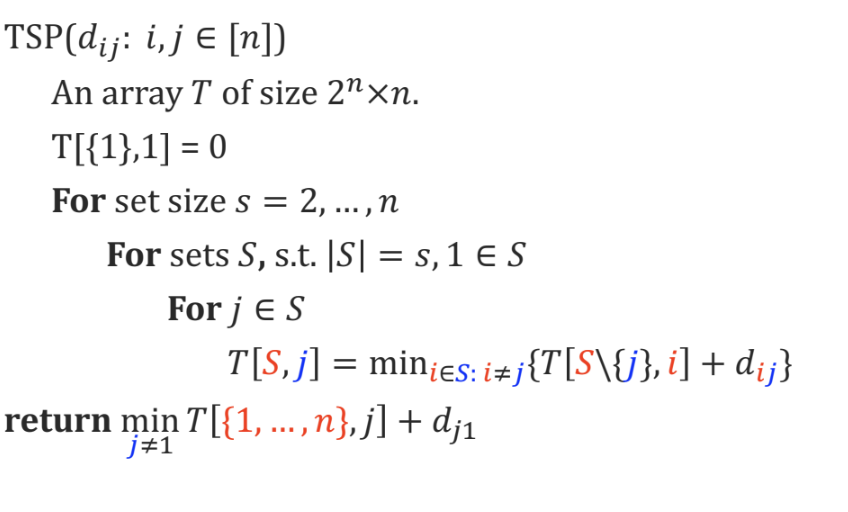
\includegraphics[scale=0.5]{TSP-code.png}
		\end{center}
	\item For runtime, there are $O(2^n \times n)$ subproblems, and on each layer we're doing $O(n)$ work, since
		we're checking the minimum across $n$ nodes every iteration. So, we have $O(n^2 2^n)$ as 
		the final runtime. 

		\question{How do we explain that \(n^2 2^n\) is the number of subproblems?}

		\answer{$O(n)$ work at every step, then $n \times 2^n$ subproblems. There are $2^n$ subsets, and in 
			each subset we can choose a $j$ to exclude, which we can upper bound by saying that there are $n$ 
		of these. So $n \times 2^n$ is a tight upper bound on the number of subproblems.}
\end{itemize}
\subsection{Independent Sets in Trees}
\begin{itemize}
	\item We're given an undirected graph \(G = (V, E)\), and want to output the largest independent 
		set of \(G\).
	\item Recall that a set \(S \subseteq V\) is considered independent if there are no 
		edges between \(u, v \in S\).
	\item This is also a notoriously hard problem, for general graphs. There isn't a polynomial time algorithm 
		that does this. But for trees, we're in luck!

		\question{Why isn't the solution just selecting every other layer?} 

		\answer{There are instances where we can pick from two consecutive layers and still not have an edge. 
		Consider the tree:
			\begin{center}
				\begin{tikzpicture}
					  \node {A}
					child {node {B}}
					child {node {C}}
					child {node {D}
					  child {node {E}}
					  child {node {F}}
					};
				\end{tikzpicture}
			\end{center}
			Our greedy algorithm would select either \(\{A, E, F\} \) or \( \{ B,C,D\} \), but the optimal set
			is actually 
		\(\{B, C, E, F\} \), so this proves that our algorithm isn't optimal.}
	\item For trees, we know that they don't have cycles, so we can pick any node and say that that is the root.
		By doing this, we can get a ``natural ordering'' of the subproblems. 
\end{itemize}

\subsubsection{Subproblems}
\begin{itemize}
	\item Let \(I(v)\) be the size of the maximum independent set in the subtree that is rooted at \(v\). 
	\item Why is this a good subproblem? Becuase it's easy to write a recursion relation for it!
	\item For the subproblems, there are two cases:

		\textit{Case 1:} \(v\) (the root of the tree) is part of the optimal independent set. This 
		means that the children aren't allowed to be part of the independent set. So if we take $v$, we can't 
		take any of the subproblems. So we need to look instead at the \textit{grandchildren} of \(v\) to join.
		Here, we'd write this as:
		\[
			I(v) = 1 + \sum_{u\  \in \text{ grandchildren}} I(u)
		\] 
		We add 1 here because we're including \(v\) now. 

		\textit{Case 2:} \( v\) is not part of the optimal independent set. Here, we would just take 
		the maximum of the children. Then:
		\[
			I(v) = \max_{u \ \in \text{ children}} \{I(u)\} 
		\] 


		So we'll take the max of these two cases:
		\[
		I(v) = \max \{1 + \sum_{u \ \in \text{ grandchildren}} I(u), \sum_{u \ \in \text{ children}} I(u)\}
		\] 
		Also, base cases is that $I(\text{leaf}) = 1$. 
\end{itemize}
\subsubsection{Implementation}
\begin{itemize}
	\item We need a data structure to store the tree easily, and also make sure that every child is processed 
		before the parents are. Well, we can iterate through the graph in post decreasing post order! 
	\item The runtime of DFS on trees is \(O(|V|)\), and each edge is looked at \(\le 2\) times -- once 
		for the children and also once for its grandchildren, so each subproblme takes constant time. 
	\item So that the total work is \(O(|E|) = O(|V|)\), since \(|E| = |V| - 1\).
\end{itemize}
